\documentclass[12pt]{article}
\usepackage[a4paper, portrait, margin=1cm, bottom=2cm]{geometry}
\usepackage{fontspec}
\usepackage[fleqn]{amsmath}
\usepackage{amssymb}
\usepackage{graphicx}
\usepackage{indentfirst}
\usepackage{polyglossia}
\usepackage[dvipsnames]{xcolor}
\usepackage{svg}

\setmainfont[Ligatures=TeX]{Times New Roman}
\newfontfamily\cyrillicfont{Times New Roman}[Script=Cyrillic]
\setdefaultlanguage{russian}
\setotherlanguages{english}
\graphicspath{graphics}

\begin{document}

\section{15. Префиксные коды.Неравенство Крафта.Алгоритм Хаффмана.}
\subsection{Префиксные коды}
$A = {a_1, \dots, a_n}$ - алфавит $ n \leq2^k\rightarrow$ 
$\begin{cases}
   a_1  \sim \underbrace{0\dots0}_{\text{k}} - c_1 \\
      a_2  \sim \underbrace{0\dots0}_{\text{k}}1 - c_2 \\
      \dots
   \end{cases}$
   \newline$l_1=l_2=l_k$ ; $M:a_{i_1},a_{i_2},\dots,a_{i_s}$ ; $\alpha=ks\geq s\log{n}$

\textbf{Шеннон-Фано}

aabc

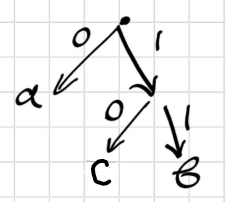
\includegraphics[width=20mm]{images/tree1.png}

$\underbrace{0}_{\text{a}}\underbrace{0}_{\text{a}}\underbrace{11}_{\text{b}}\underbrace{01}_{\text{c}}$

$\begin{cases}
   a  \sim 0 \\
      b  \sim 11 \\
      c \sim 01
   \end{cases}$

\subsubsection{Определение}
Код называется \textit{префиксным}, если ни одно кодовое слово не является началом другого кодового слова. 

\subsection{Неравенство Крафта}
Для префиксного кода с длинами $l_1,\dots,l_s$

$\sum\limits_{i=1}^s 2^{-l_i} \leq 1$
\subsubsection{Доказательство}
$l_1\leq l_2 \leq \dots \leq l_s=q$ 

$A_i=\{\underbrace{(\dots)}_{\text{q двоичных чисел}})|$нач. с $l_i\}$

$A_i\cap A_j=\emptyset$

\subsubsection{Замечание}
$\cup A_i \leq \{ \underbrace{(\dots)}_{\text{q раз p}}\}$

$\sum\limits_{i=1}^s 2^{q-l_i} \leq 2^q$
\subsubsection{Теорема}
$p_1,\dots, p_n$ - вер, с которой встречаются $a_1, \dots, a_n$

Сред. длин. код. слова $L = \sum\limits_{i=1}^n l_ip_i $ ; $L \geq H(p_1, \dots, p_s)$
\subsubsection{Доказательство}
$\sqsupset q_i=\frac{2^{-l_i}}{\sum\limits_{i=1}^n2^{l_i}}$ ; $L-H(p_1,\dots, p_n)=\sum\limits_{i=1}^nl_ip_i+\sum\limits_{i=1}^np_i\log\limits_2{p_i}=\sum\limits_{i=1}^np_i\log\limits_2(p_i2^{l_i})=$

$=\sum\limits_{i=1}^np_ilog{\frac{p_i}{2^{-l_i}}} \geq \sum\limits_{i=1}^np_i\log\limits_2{\frac{p_i\sum\limits_{j=1}^n2^{-l_j}}{2^{-l_i}}}=\sum\limits_{i=1}^np_i\log\limits_2{\frac{p_i}{q_i}}=D(p||q) \geq 0$

$\rightarrow L \geq H(p_1, \dots, p_n) + D(p||q)$
\subsection{Алгоритм Хаффмана}

$a_1, \dots, a_n$ c $p_1, \dots, p_n$

$p_i = \frac{N(a_i)}{N}$

$p_1, p_2, \dots, p_s$

$p_i \geq p_j \rightarrow l_i \leq l_j$

$\sum\limits_{i=1}^s 2^{-l_i} \leq 1 (*)$

$p_{n-1}, p_n$ - наим.вер $\rightarrow l_{n-1} = l_n$

[чтобы знам $(*)$ сокращался]
\subsubsection{Пример}
$\underbrace{a \sim 0,22 \text{ ; }b \sim 0,2}_{ab \sim 0,42}$ ; $c \sim 0,15$; $\underbrace{d \sim 0,13 \text{ ; }e \sim 0,12}_{de \sim 0,25}$ ; $\underbrace{f \sim 0,1\text{ ; } g \sim 0,18 }_{fg \sim 0,18}$

$\underbrace{cfg \sim 0,33 \text{ ; }de \sim 0,25}_{cdefg \sim 0,58}$ ; $ab \sim 0,42$

$\underbrace{ab \sim 0,42 \text{ ; }cdefg \sim 0,58}_{abcdefg \sim 1}$

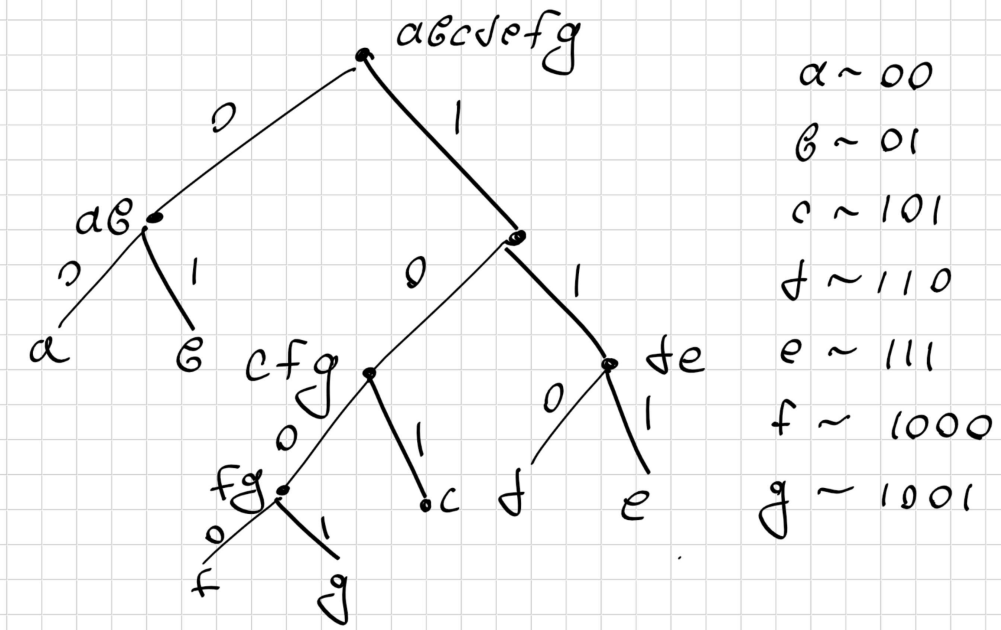
\includegraphics[width=100mm]{images/tree2.png}
\end{document}